\documentclass[a0paper,portrait,margin=18mm]{tikzposter}
\input{socceranalytics} % configure for poster session

\usepackage{booktabs}
\usepackage{graphicx}
\usepackage{array}

% identify your project and choose a main color
% =================================================================
\project{B7}{NAP}{AD}
\students{%
  Ada Batu Yildirim,
  Irem Gabay,
  Can Goktan,
  Esteban Schmid,
  Deniz Utku Akbas
 }
\maincolor{petrol}
% =================================================================

\newcommand{\figcap}[1]{\vspace{2mm}{\small\textit{#1}}}

% =================================================================
\begin{document}\maketitle
% =================================================================

\block{Research question: does Napoli's attacking possession justify its defensive risk?}
{
\large
\Large
We study Napoli's Champions League league-phase matches using StatsBomb event data.
The poster follows the chain from \textbf{attacking access} to \textbf{chance quality}
to \textbf{transition defence}. Napoli's profile is not simply good or bad:
they enter advanced zones often enough, but the value created from those entries is modest,
and the team becomes vulnerable when attacks break down.

\medskip
\begin{tabular}{>{\bfseries}p{0.18\linewidth}p{0.78\linewidth}}
Headline &
Napoli rank \textbf{9th} for passes into the box, but only \textbf{27th} for xG per match
and \textbf{29th} for xG per shot. The ball gets close to goal more often than the final
shot quality suggests.\\
Risk trade-off &
Ball losses become opponent shots within 30 seconds at \textbf{6.5\%}, versus a same-match
league baseline of \textbf{3.8\%}. Napoli therefore pay a relatively high defensive price
for attacks that are not yet high-value enough.\\
Poster message &
Improve the last connection in attack while protecting the spaces behind the ball.
The tactical fix is not less possession; it is more purposeful possession with better
rest-defence.
\end{tabular}
}

\begin{columns}

\column{0.33}

\block{1. Attack benchmark: entries are better than end product}
{
\centering
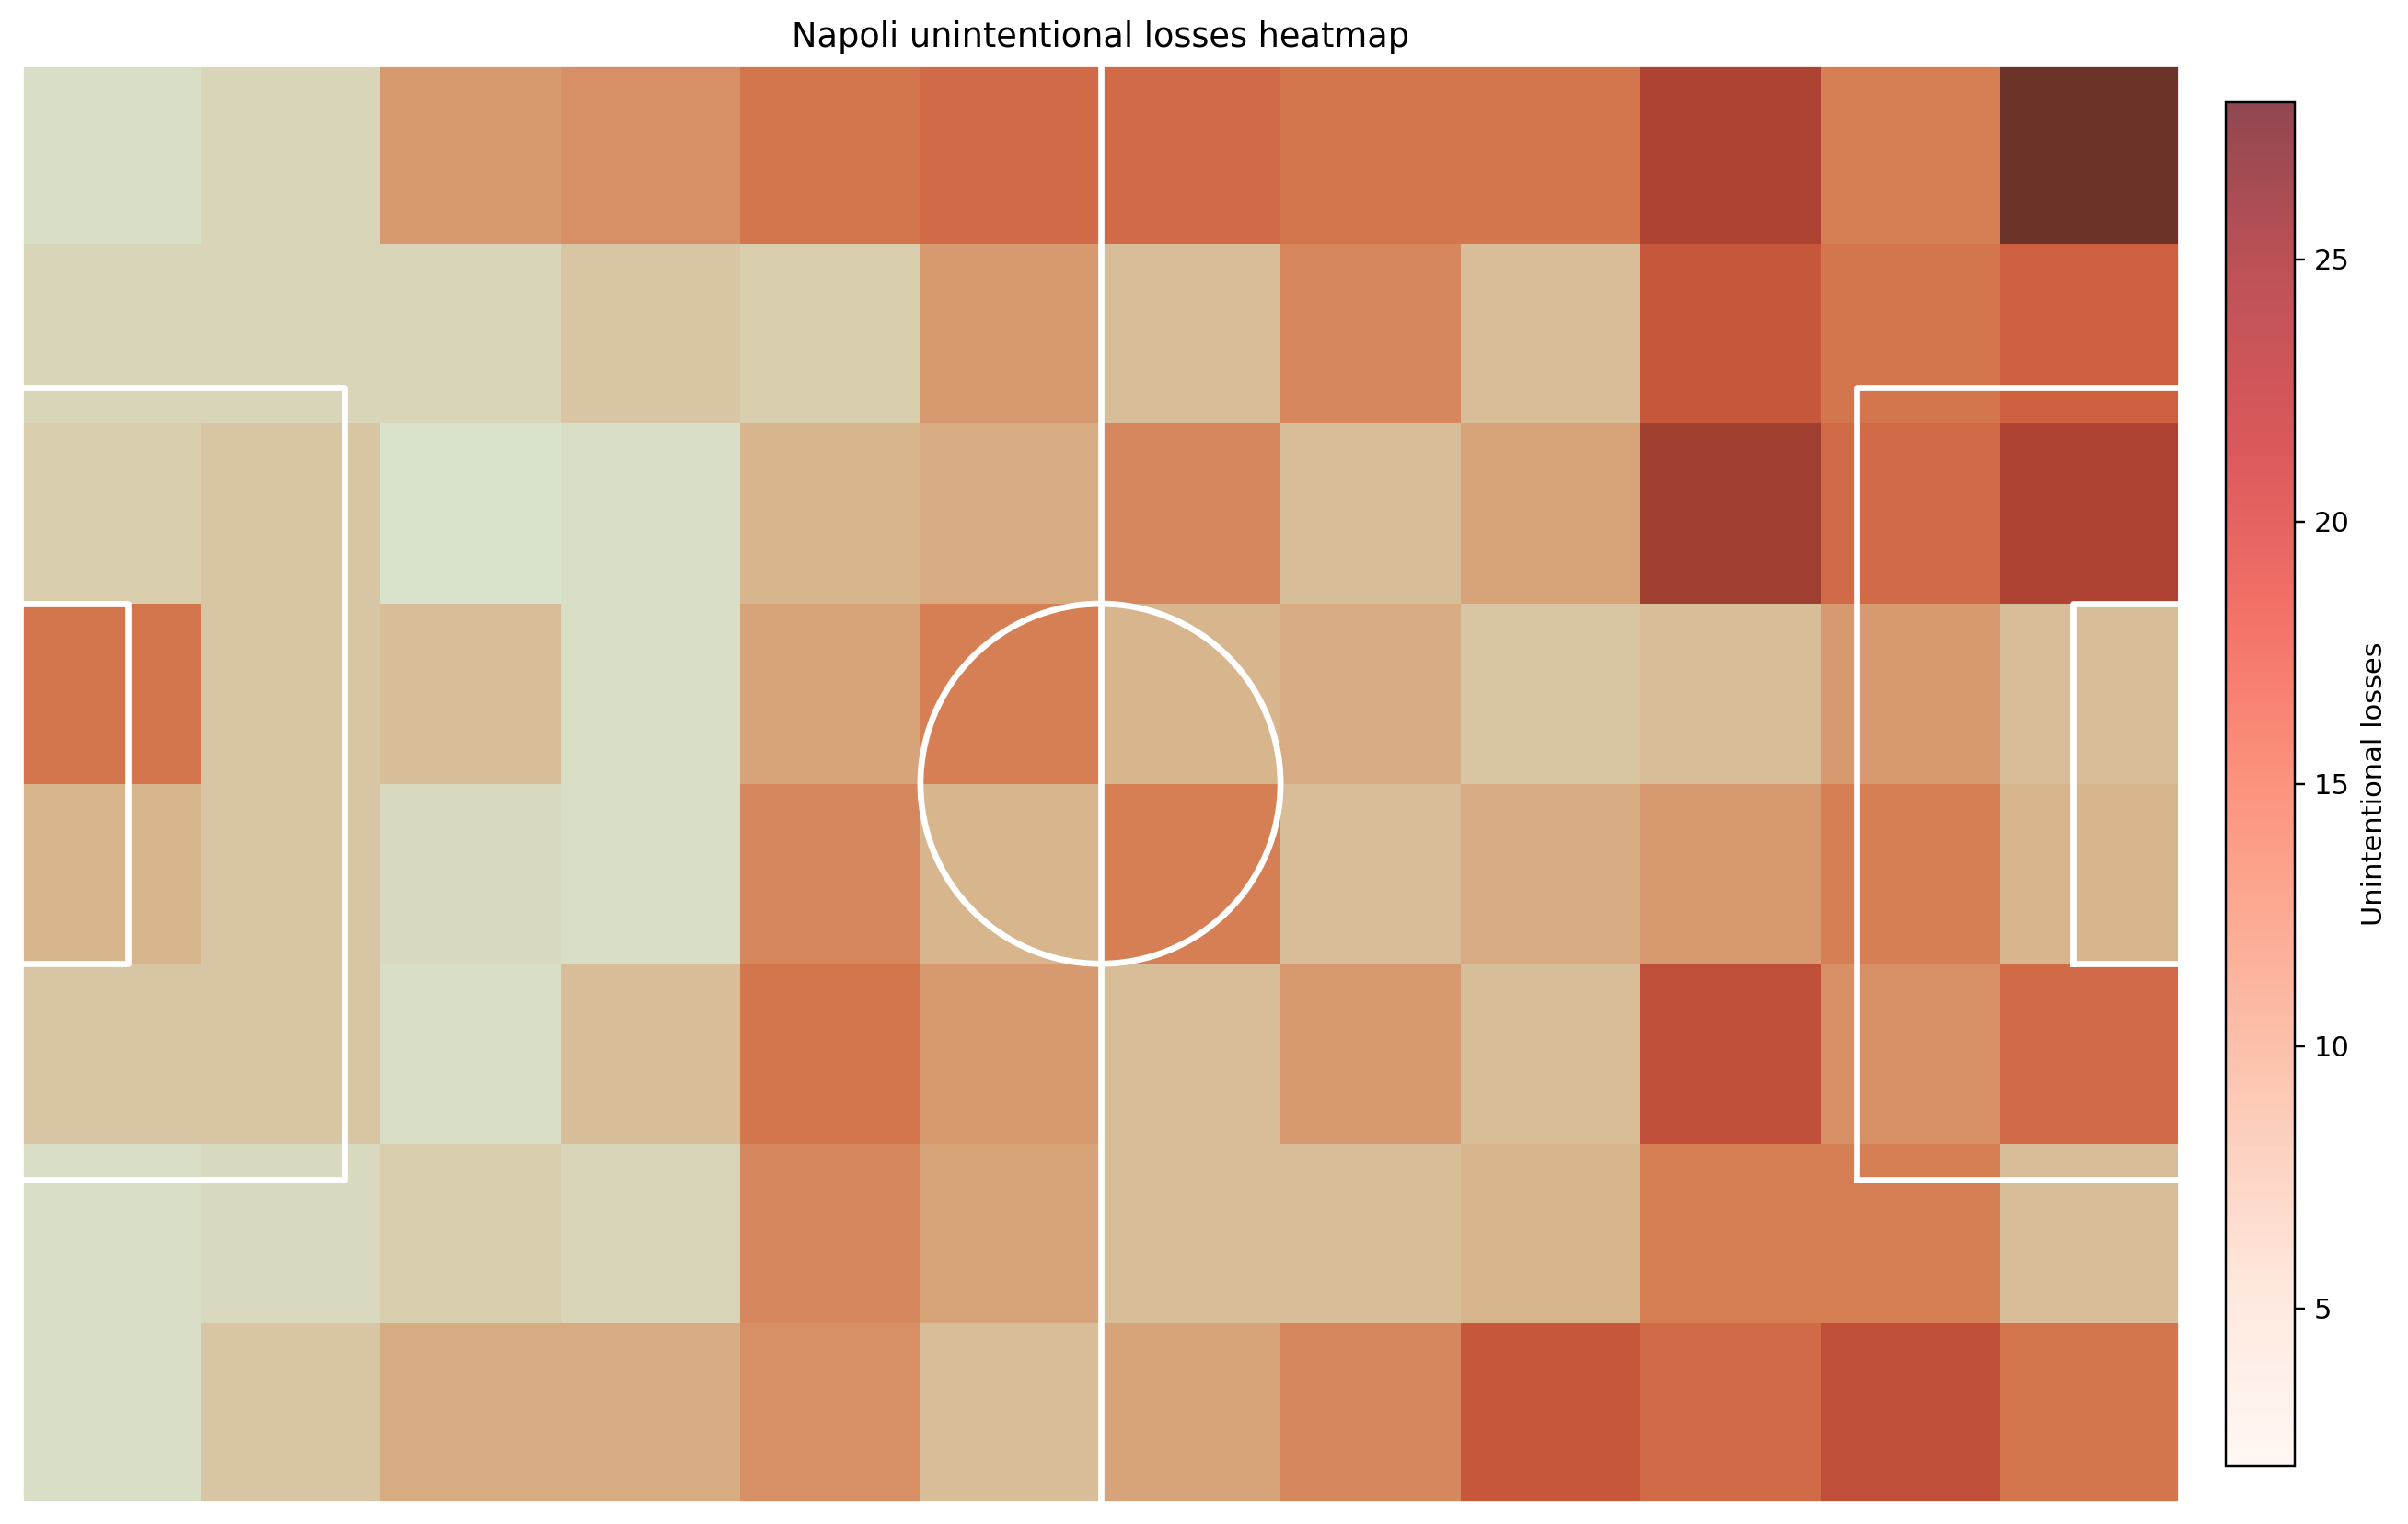
\includegraphics[width=\linewidth]{poster_attack_radar}

\figcap{Radar percentiles against other teams. Napoli's entry metrics are healthier than their shot-value and OBV profile.}

\medskip
\normalsize
\begin{tabular}{lr}
\toprule
Headline metric & Napoli\\
\midrule
xG per match & 1.15 \quad (27th)\\
Shots per match & 11.88 \quad (25th)\\
xG per shot & 0.097 \quad (29th)\\
Touches in box per match & 78.88 \quad (14th)\\
Passes into box per match & 16.63 \quad (9th)\\
Progressive passes per match & 122.13 \quad (11th)\\
OBV per match & 0.85 \quad (34th)\\
\bottomrule
\end{tabular}

\medskip
\normalsize
The table explains the radar shape. Napoli can move the ball forward and access the box,
but the attack loses value at the final action. A team with top-ten box-entry volume should
not sit in the bottom third for xG per shot unless many attacks end from poor angles,
crowded central zones, or rushed decisions. This is the key attacking mismatch: Napoli
look territorially competitive, but their final actions do not create enough expected goals.
}

\block{2. Shot map: access exists, clean shots are the bottleneck}
{
\centering
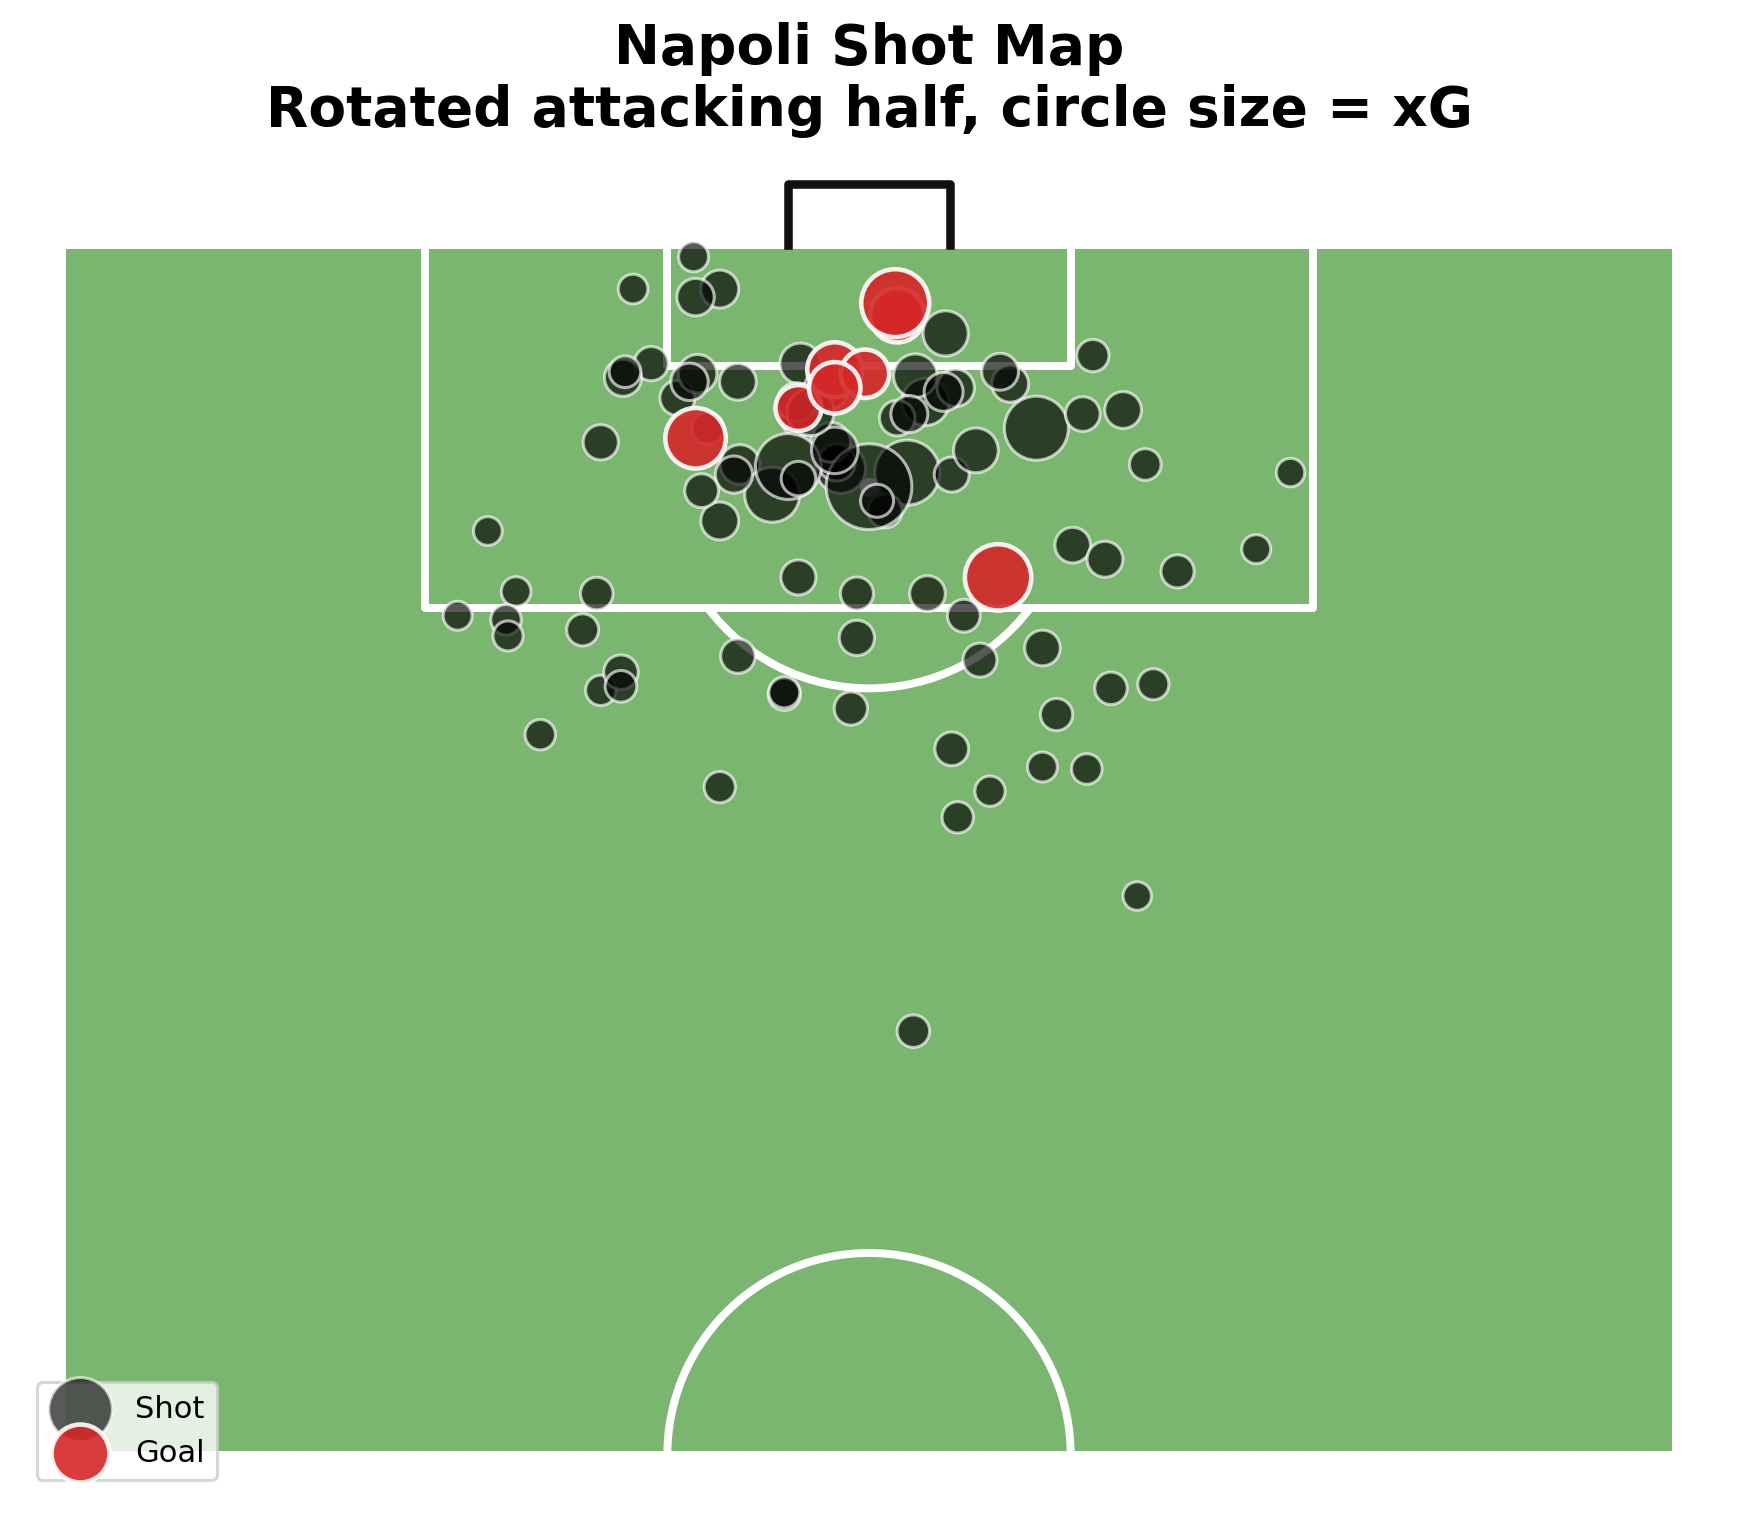
\includegraphics[width=0.96\linewidth]{poster_shot_map}

\figcap{Rotated attacking-half shot map. Napoli produced 95 shots and 9.17 xG; average shot quality was 0.097 xG per shot.}

\smallskip
\normalsize
The shot map supports a measured interpretation: Napoli do not fail to arrive. They fail
to turn enough arrivals into high-probability shots. Several attempts are either outside the
highest-value central corridor or taken after the defence has recovered. The recommendation is
to favour cut-backs, central lay-offs, and third-player arrivals over early speculative shots.
In practical terms, the attack needs one more pass or one more support run before the shot,
not simply more shots.
}

\column{0.34}

\block{3. Passing: stable circulation, sharper creation needed}
{
\normalsize
\begin{tabular}{lr}
\toprule
Passing metric & Napoli\\
\midrule
Total passes & 4,460\\
Completion rate & 85.3\%\\
Under pressure completion & 75.3\%\\
No pressure completion & 87.4\%\\
Progressive passes & 1,310\\
Passes into final third & 409\\
Passes into box & 300\\
Shot assists & 69\\
Goal assists & 6\\
Lofted long balls & 374\\
\bottomrule
\end{tabular}

\medskip
\centering
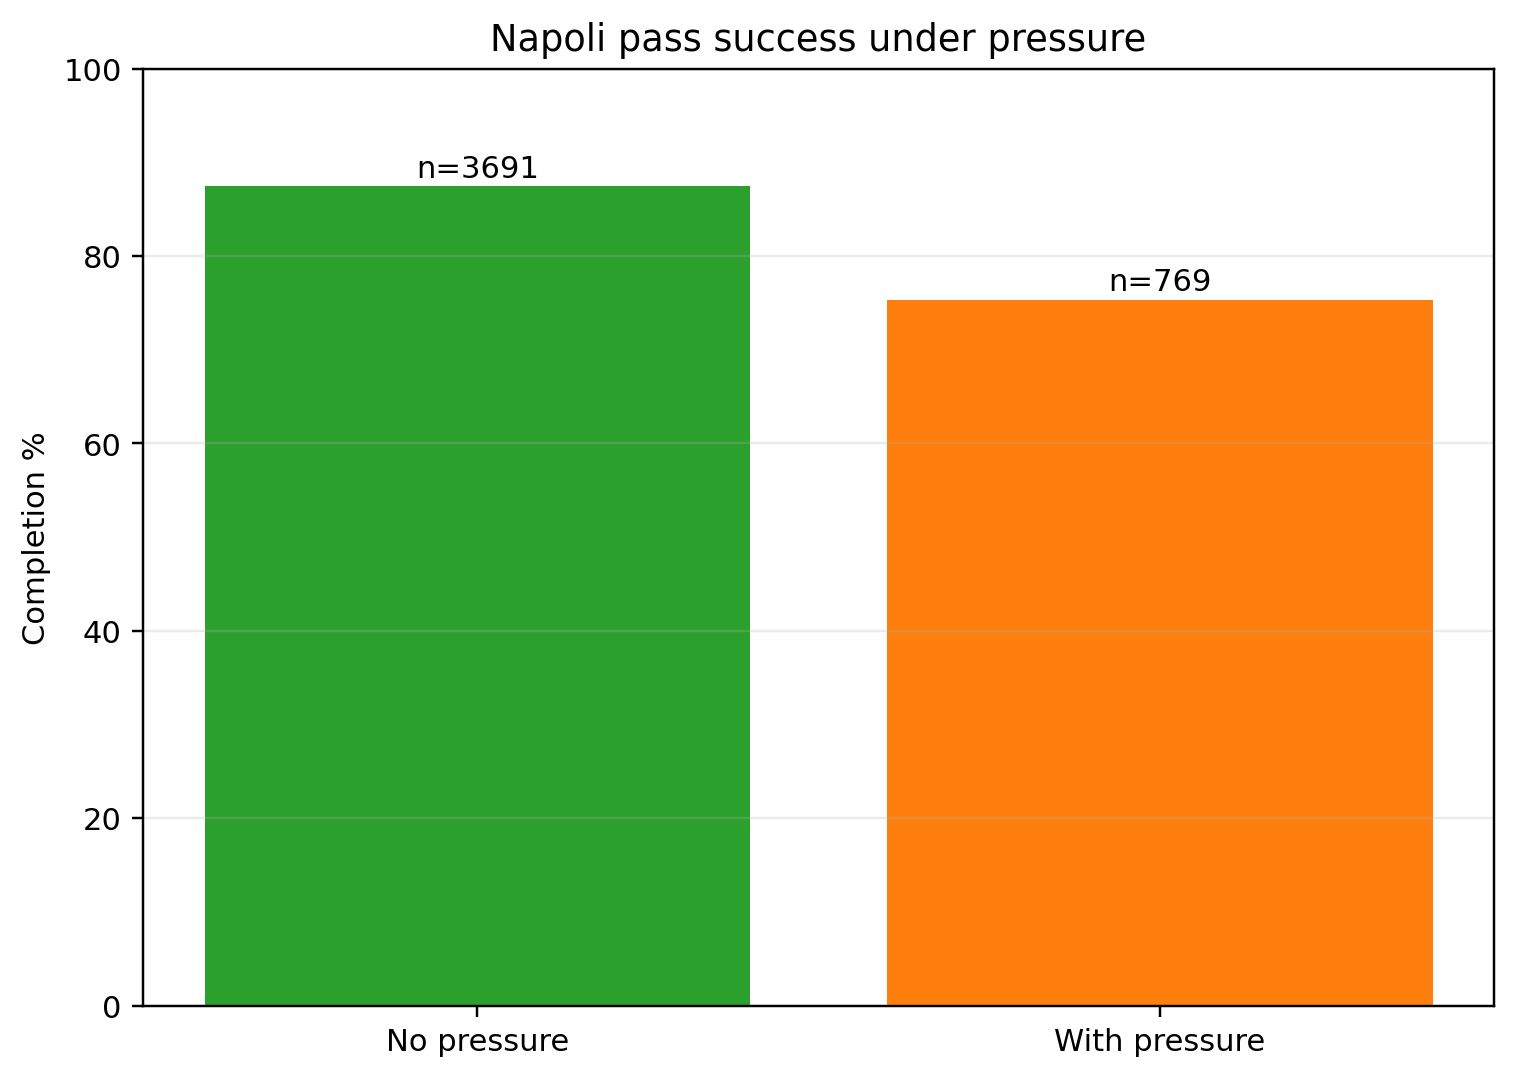
\includegraphics[width=0.98\linewidth]{poster_pressure_success}

\figcap{Pressure reduces Napoli's pass completion by about 12 percentage points.}

\medskip
\normalsize
This does not describe a team that cannot pass. It describes a team whose possession becomes
less reliable under pressure, especially when the next pass must progress play. Better support
angles around the ball would let Napoli keep the same attacking ambition with fewer emergency
clearances, rushed long balls, and uncontrolled turnovers. The pressure split also helps explain
why possession can look controlled for long phases but still break down sharply near the box.
}

\block{4. Where possession is efficient}
{
\centering
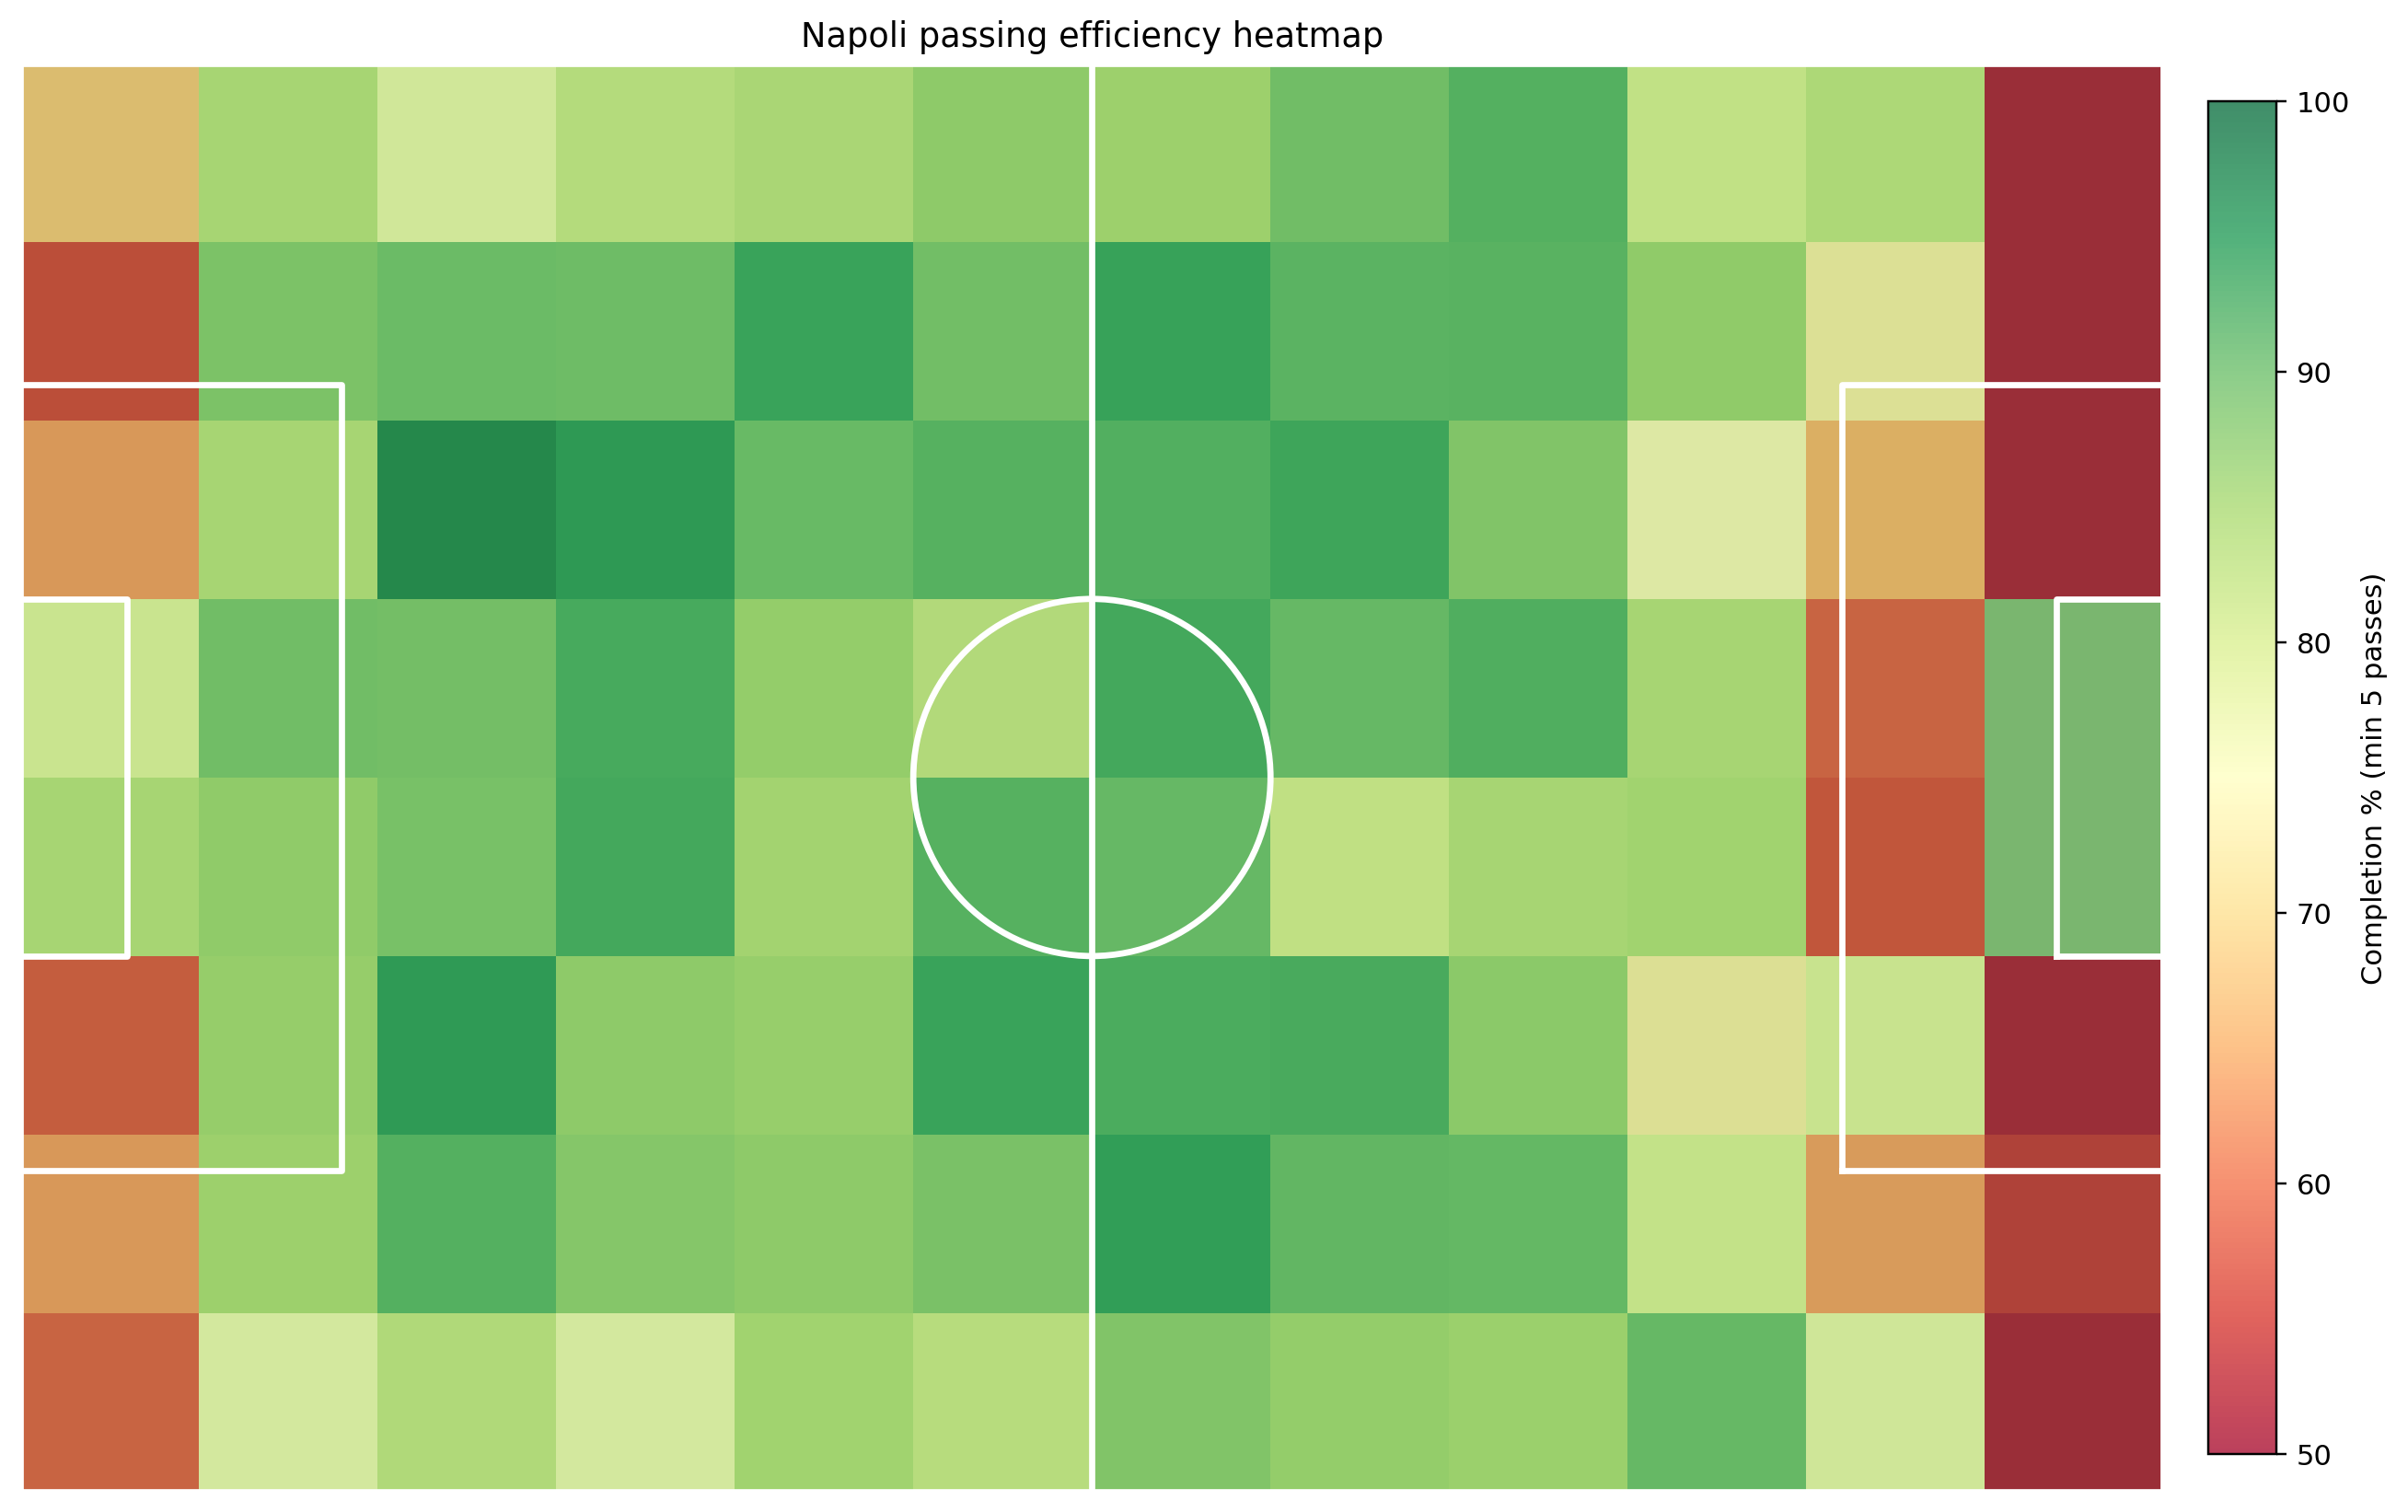
\includegraphics[width=\linewidth]{poster_pass_efficiency}

\figcap{Passing efficiency by larger pitch zones. Larger squares reduce noise and make the stable/risky areas easier to read.}

\smallskip
\normalsize
The efficiency map helps separate harmless circulation from useful possession. Napoli's stable
zones are mostly deeper and wider. Near the box, where passes should create the final advantage,
efficiency becomes more fragile. This is exactly where the attack-to-defence trade-off matters:
failed final-third passes become transition moments against a stretched team. Napoli should keep
the progression volume, but make the final-third structure less dependent on isolated receivers.
}

\column{0.33}

\block{5. Defensive transition: losses are too dangerous}
{
\centering
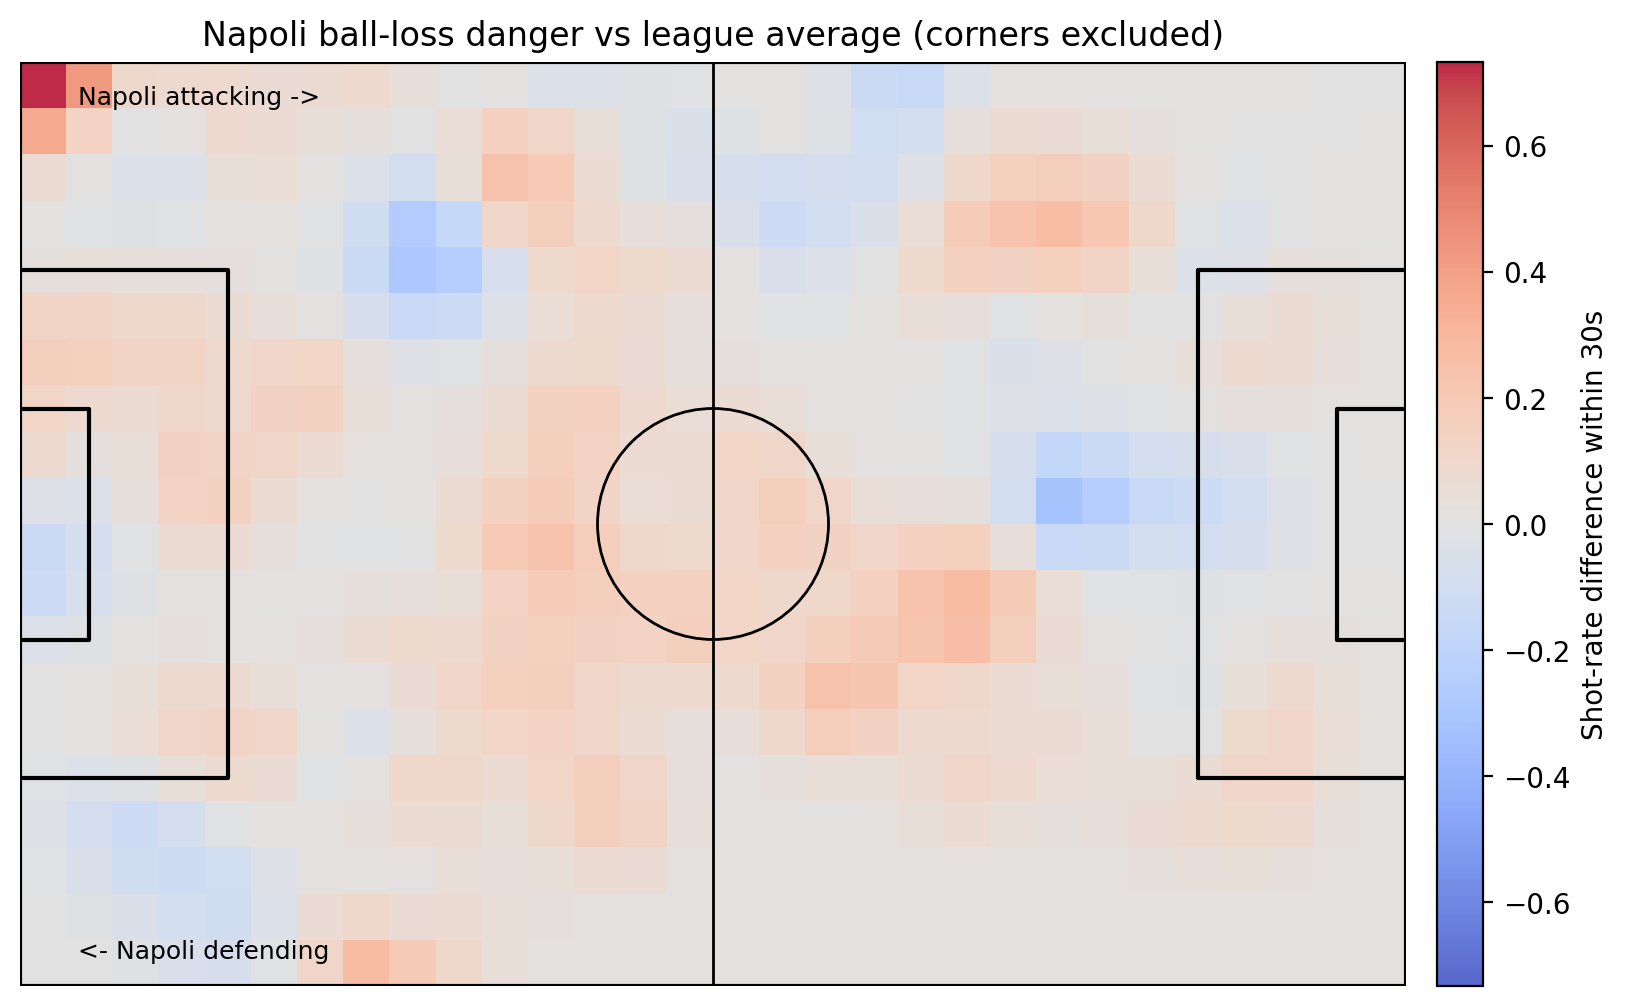
\includegraphics[width=\linewidth]{poster_loss_danger_vs_average}

\figcap{Diverging heatmap of ball-loss danger vs the same-match league average. Corners are excluded.}

\medskip
\normalsize
\begin{tabular}{lrr}
\toprule
Transition metric & Napoli & League\\
\midrule
Pressures / match & 154.75 & 190.50\\
Recoveries / match & 41.75 & 40.75\\
Interceptions / match & 4.50 & 7.12\\
Ball losses / match & 106.25 & 102.50\\
Loss-to-shot rate & 6.5\% & 3.8\%\\
Recovery time & 7.98s & 7.52s\\
\bottomrule
\end{tabular}

\medskip
\normalsize
Napoli recover the ball at roughly league-average volume, but they pressure less and intercept
less. That matters because their attacks often end with players already committed ahead of the
ball. When the first counter-pressure action fails, the opponent can move directly into a shot
window more often than the baseline. The solution is not only defensive effort; it is spacing.
The player behind the attack must be close enough to delay the first forward pass after a turnover.
}

\block{Recommendations}
{
\small
\begin{enumerate}
\item \textbf{Create cleaner central shots.} Keep the box-entry volume, but bias final actions
toward cut-backs, central wall passes, and late arrivals instead of early low-value shots.
\item \textbf{Add pressure-proof support.} The 12-point completion drop under pressure means
Napoli need shorter escape routes near the ball before the risky pass is played.
\item \textbf{Set rest-defence before crossing or shooting.} If both wide players attack the box,
one midfielder should hold an interception lane. Napoli's loss-to-shot rate is nearly double
the same-match baseline.
\item \textbf{Reduce unforced bad passes, not attacking ambition.} The report counts 654 bad
passes and 374 lofted long balls. The goal is fewer unstable passes, not fewer attempts to progress.
\end{enumerate}
}

\block{Conclusion}
{
\small
Napoli's possession has enough territory to be useful, but it currently leaves too much value
on the table. The attack reaches the box, yet shot quality and OBV lag behind. At the same time,
turnovers expose a rest-defence structure that pressures and intercepts less than comparable
teams in the same matches. The best tactical path is therefore two-sided: \textbf{raise chance
quality without lowering attacking volume, and organise the next defensive action before the
attack is lost}.
}

\end{columns}

% =================================================================
\end{document}
% =================================================================
